Encontrar la matriz de transformación que produce un giro de 120 grados a un sistema de 
coordenadas rectangular en torno a un eje fijo (expresar sobre que eje se hace el giro). 
Los ejes coordenados son perpendiculares entre sí.\\

\textbf{Rotación de $\theta = 120^\circ$ alrededor del eje $x_{2}$.}\\
Utilizando cosenos directores para representar la matriz de transformación:

\begin{figure*}[h]
    \centering
    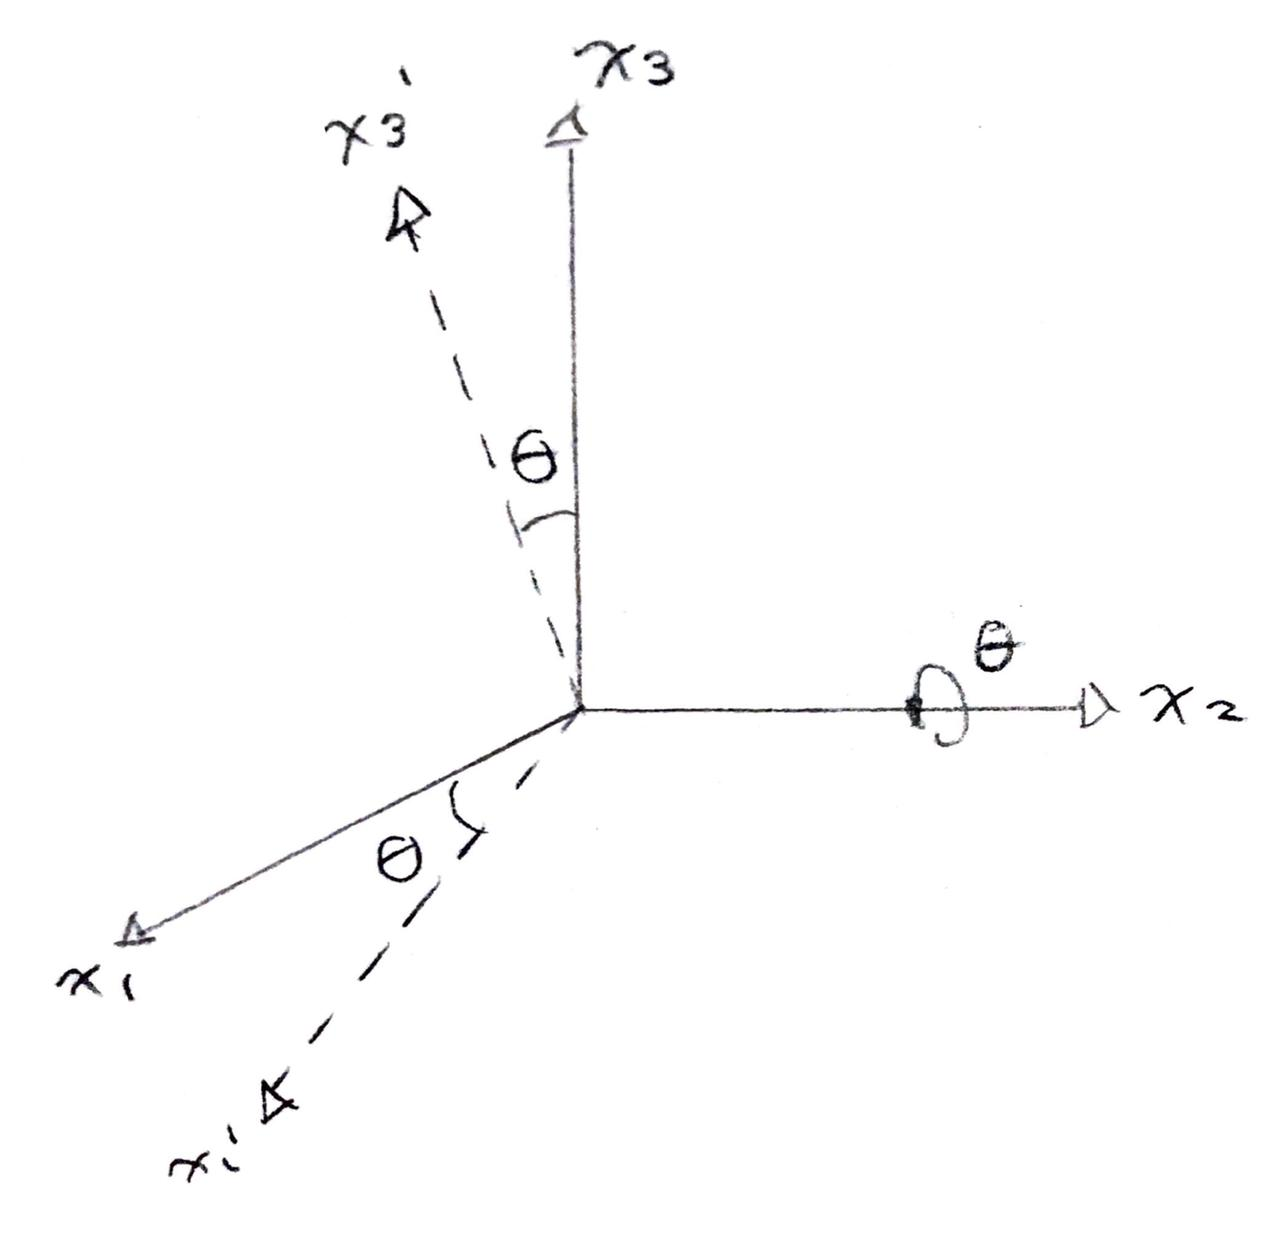
\includegraphics[scale=0.15]{eje_coordenado.jpeg}
\end{figure*}

\begin{align*}
    \lambda_{11} &= \cos(x'_{1},x_{1}) = \cos(\theta) \\
    \lambda_{12} &= \cos(x'_{1},x_{2}) = \cos\left(\frac{\pi}{2}\right) = 0 \\
    \lambda_{13} &= \cos(x'_{1},x_{3}) = \cos\left(\frac{\pi}{2}+\theta\right) = -\sin(\theta) \\
    \lambda_{21} &= \cos(x'_{2},x_{1}) = \cos\left(\frac{\pi}{2}\right) = 0 \\
    \lambda_{22} &= \cos(x'_{2},x_{2}) = \cos(0) = 1 \\
    \lambda_{23} &= \cos(x'_{2},x_{3}) = \cos\left(\frac{\pi}{2}\right) = 0 \\
    \lambda_{31} &= \cos(x'_{3},x_{1}) = \cos\left(\frac{\pi}{2}-\theta\right) = \sin(\theta) \\
    \lambda_{32} &= \cos(x'_{3},x_{2}) = \cos\left(\frac{\pi}{2}\right) = 0 \\
    \lambda_{33} &= \cos(x'_{3},x_{3}) = \cos(\theta) 
\end{align*}

Entonces la matriz de transformación queda:
\vspace{5 mm}
\begin{equation*}
    \lambda = \begin{bmatrix}
        \cos(\theta) & 0 & -\sin(\theta) \\
        0 & 1 & 0 \\
        \sen(\theta) & 0 & \cos(\theta)
       \end{bmatrix}
    = \begin{bmatrix}
        \cos(120^\circ) & 0 & -\sen(120^\circ) \\
        0 & 1 & 0 \\
        \sen(120^\circ) & 0 & \cos(120^\circ)
    \end{bmatrix}
\end{equation*}

\vspace{5 mm}
\begin{equation*}
    \therefore \lambda = \begin{bmatrix}
        -\frac{1}{2} & 0 & -\frac{\sqrt{3}}{2} \\
        0 & 1 & 0 \\
        \frac{\sqrt{3}}{2} & 0 & -\frac{1}{2}
    \end{bmatrix}
\end{equation*}